\documentclass[standalone]{beamer}

\begin{document}
\section{進階線段樹}

\begin{frame}[fragile]{進階線段樹}
  \begin{itemize}
    \item 來看看強大的線段樹可以做些什麼吧~
    \item 這裡講的技巧只是線段樹強大應用中的冰山一角,有興趣的讀者可以閱讀進階資料結構講義,或者是自行上網搜尋更加進階的應用喔!
  \end{itemize}
\end{frame}

\begin{frame}[fragile]{\btitle{精妙狀態合併}}
  \begin{itemize}
    \item 線段樹不僅可以維護簡單的最大最小值或總和,只要能夠快速從左右子區間的資訊得知合併後的區間的所有資訊的問題,就可以用線段樹解決
    \item 來看例題!
    \begin{problem}[區間最大連續和]
      給定長度為 \(N\) 的序列 \(a_1, a_2, \dots, a_N\),接著有 \(Q\) 個形如 \(\texttt{l r}\) 的詢問,請你回答 \(a_l, a_{l+1}, \dots, a_r\) 這個序列的最大連續和。

      \begin{itemize}
          \item
              \(N, Q \leq 5 \times 10^5\)
      \end{itemize}
    \end{problem}
  \end{itemize}
\end{frame}

\begin{frame}[fragile]{\btitle{精妙狀態合併}}
  \begin{itemize}
    \item 想想看怎麼用分治法求出最大連續和!
    \item 在線段樹每個節點上,我們可以維護以下資訊:
      \begin{itemize}
          \item 以區間最左端為左界的最大連續和,即最大總和的前綴。
          \item 以區間最右端為右界的最大連續和,即最大總和的後綴。
          \item 整個區間的最大連續和。
          \item 整個區間的總和。
      \end{itemize}
    \item 所有的區間可以分成三種:通過區間中點、完全落在左半區間、完全落在右半區間
    \item 中點的最大連續和一定是左半區間的最大後綴加上右半區間的最大前綴
  \end{itemize}
\end{frame}

\begin{frame}[fragile]{\btitle{精妙狀態合併}}
  \begin{minted}[breaklines]{cpp}
    struct Info {
      int64_t sum, lmx, rmx, mx;
    };
    Info combine(const Info &lhs, const Info &rhs) {
      Info res;
      res.sum = lhs.sum + rhs.sum;
      res.lmx = max(lhs.lmx, lhs.sum + rhs.lmx);
      res.rmx = max(lhs.rmx + rhs.sum, rhs.rmx);
      res.mx = max({lhs.mx, rhs.mx, lhs.rmx + rhs.lmx});
      return res;
    }
  \end{minted}
\end{frame}

\begin{frame}[fragile]{\btitle{懶人標記}}
  \begin{itemize}
    \item 直接來看例題!
    \begin{problem}[區間加值、區間最大值]
      給定一個長度為 \(N\) 的正整數序列 \(a_1, \dots, a_N\),接著有 \(Q\) 個詢問,每個詢問形如
      \begin{itemize}
          \item
              \(\texttt{1 l r}\),請輸出 \(a_l, a_{l+1}, \dots, a_r\) 當中最大的數字是多少。
          \item
              \(\texttt{2 l r d}\),讓 \(a_l, a_{l+1}, \dots, a_r\) 全部增加 \(d\)。
      \end{itemize}

      \begin{itemize}
          \item \(N, Q \leq 5 \times 10^5\)
          \item \(d > 0\)
      \end{itemize}
    \end{problem}
  \end{itemize}
\end{frame}

\begin{frame}[fragile]{\btitle{懶人標記}}
  \begin{itemize}
    \item 如果這題只是單純做 $r - l + 1$ 次單點修改的話,修改的複雜度會退化成 $O(N \log N)$
    \item 有沒有辦法把修改的區間拆成 $O(\log N)$ 個區間,並對每個區間做一些事情後,就達到修改的效果呢?
    \item 可以!
  \end{itemize}
\end{frame}

\begin{frame}[fragile]{\btitle{懶人標記}}
  \begin{itemize}
    \item 每個節點上面存一個「標記」,表示被\textbf{這個節點對應的區間涵蓋的所有元素都必須加上某個值}
    \item 在區間修改時,我們就在所有區間打上這樣的「標記」
    \item 在打標記的時候,同時修改該節點的資訊,並且一路 pull 回去!
  \end{itemize}
\end{frame}

\begin{frame}[fragile]{\btitle{懶人標記}}
  \begin{itemize}
    \item $a = [1, 16, 2, 8, 4]$,並把 $[1, 4]$ 加上 $3$
    \item 先把 tag 打上去!
      \begin{figure}
        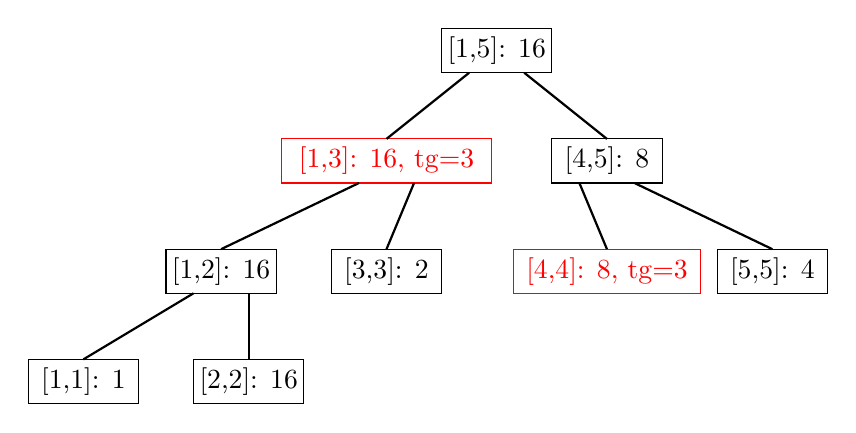
\begin{tikzpicture}[scale=0.7]
          \draw [black] (-1,7.9) rectangle (1,7.1) node [black, midway] {[1,5]: 16}; % Draws a rectangle

          \draw [red] (-3.9,5.9) rectangle (-0.1,5.1) node [red,midway] {[1,3]: 16, tg=3}; % Draws a rectangle
          \draw [black] (1,5.9) rectangle (3,5.1) node [black,midway] {[4,5]: 8}; % Draws a rectangle

          \draw [black] (-6,3.9) rectangle (-4,3.1) node [black,midway] {[1,2]: 16}; % Draws a rectangle
          \draw [black] (-3,3.9) rectangle (-1,3.1) node [black,midway] {[3,3]: 2}; % Draws a rectangle
          \draw [red] (0.3,3.9) rectangle (3.7,3.1) node [red,midway] {[4,4]: 8, tg=3}; % Draws a rectangle
          \draw [black] (4,3.9) rectangle (6,3.1) node [black,midway] {[5,5]: 4}; % Draws a rectangle

          \draw [black] (-8.5,1.9) rectangle (-6.5,1.1) node [black,midway] {[1,1]: 1}; % Draws a rectangle
          \draw [black] (-5.5,1.9) rectangle (-3.5,1.1) node [black,midway] {[2,2]: 16}; % Draws a rectangle

          \draw [thick] (-0.5,7.1) to (-2,5.9);
          \draw [thick] (0.5,7.1) to (2,5.9);

          \draw [thick] (-2.5,5.1) to (-5,3.9);
          \draw [thick] (-1.5,5.1) to (-2,3.9);

          \draw [thick] (1.5,5.1) to (2,3.9);
          \draw [thick] (2.5,5.1) to (5,3.9);

          \draw [thick] (-5.5,3.1) to (-7.5,1.9);
          \draw [thick] (-4.5,3.1) to (-4.5,1.9);
          % \draw [thick] (-2,2) % Draws a line
          % to [out=10,in=190] (2,2)
          % to [out=10,in=90] (6,0) 
          % to [out=-90,in=30] (-2,-2);    
        \end{tikzpicture}
      \end{figure}
  \end{itemize}
\end{frame}

\begin{frame}[fragile]{\btitle{懶人標記}}
  \begin{itemize}
    \item $a = [1, 16, 2, 8, 4]$,並把 $[1, 4]$ 加上 $3$
    \item 更新被打 tag 的區間的答案
      \begin{figure}
        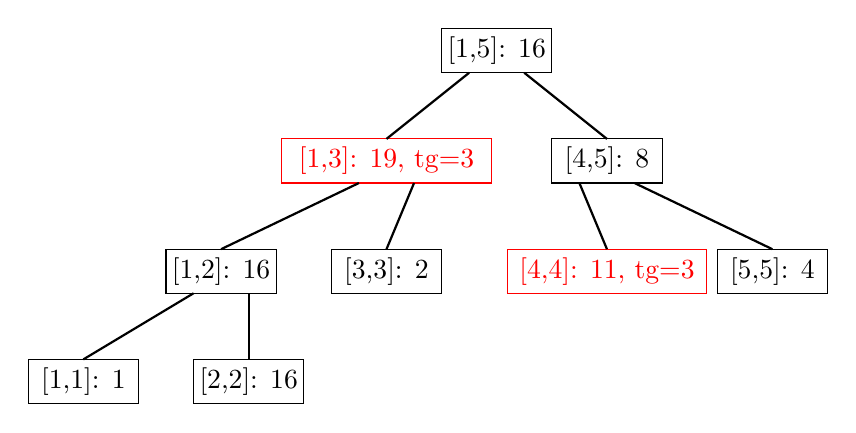
\begin{tikzpicture}[scale=0.7]
          \draw [black] (-1,7.9) rectangle (1,7.1) node [black, midway] {[1,5]: 16}; % Draws a rectangle

          \draw [red] (-3.9,5.9) rectangle (-0.1,5.1) node [red,midway] {[1,3]: 19, tg=3}; % Draws a rectangle
          \draw [black] (1,5.9) rectangle (3,5.1) node [black,midway] {[4,5]: 8}; % Draws a rectangle

          \draw [black] (-6,3.9) rectangle (-4,3.1) node [black,midway] {[1,2]: 16}; % Draws a rectangle
          \draw [black] (-3,3.9) rectangle (-1,3.1) node [black,midway] {[3,3]: 2}; % Draws a rectangle
          \draw [red] (0.2,3.9) rectangle (3.8,3.1) node [red,midway] {[4,4]: 11, tg=3}; % Draws a rectangle
          \draw [black] (4,3.9) rectangle (6,3.1) node [black,midway] {[5,5]: 4}; % Draws a rectangle

          \draw [black] (-8.5,1.9) rectangle (-6.5,1.1) node [black,midway] {[1,1]: 1}; % Draws a rectangle
          \draw [black] (-5.5,1.9) rectangle (-3.5,1.1) node [black,midway] {[2,2]: 16}; % Draws a rectangle

          \draw [thick] (-0.5,7.1) to (-2,5.9);
          \draw [thick] (0.5,7.1) to (2,5.9);

          \draw [thick] (-2.5,5.1) to (-5,3.9);
          \draw [thick] (-1.5,5.1) to (-2,3.9);

          \draw [thick] (1.5,5.1) to (2,3.9);
          \draw [thick] (2.5,5.1) to (5,3.9);

          \draw [thick] (-5.5,3.1) to (-7.5,1.9);
          \draw [thick] (-4.5,3.1) to (-4.5,1.9);
          % \draw [thick] (-2,2) % Draws a line
          % to [out=10,in=190] (2,2)
          % to [out=10,in=90] (6,0) 
          % to [out=-90,in=30] (-2,-2);    
        \end{tikzpicture}
      \end{figure}
  \end{itemize}
\end{frame}

\begin{frame}[fragile]{\btitle{懶人標記}}
  \begin{itemize}
    \item $a = [1, 16, 2, 8, 4]$,並把 $[1, 4]$ 加上 $3$
    \item pull 回 root!
      \begin{figure}
        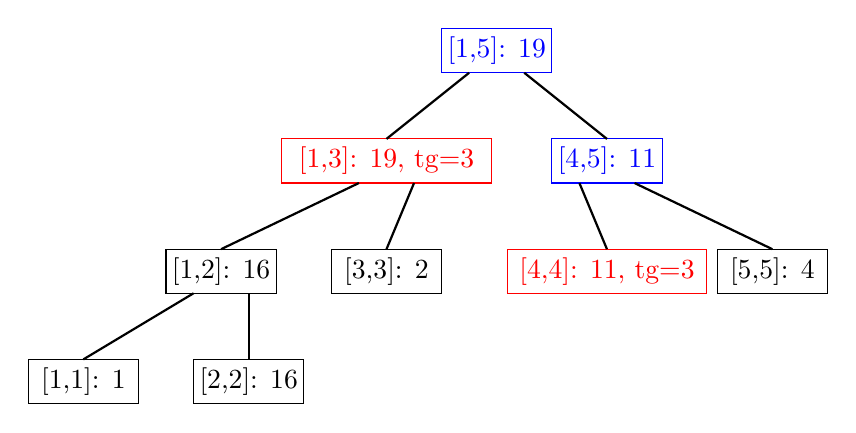
\begin{tikzpicture}[scale=0.7]
          \draw [blue] (-1,7.9) rectangle (1,7.1) node [blue, midway] {[1,5]: 19}; % Draws a rectangle

          \draw [red] (-3.9,5.9) rectangle (-0.1,5.1) node [red,midway] {[1,3]: 19, tg=3}; % Draws a rectangle
          \draw [blue] (1,5.9) rectangle (3,5.1) node [blue,midway] {[4,5]: 11}; % Draws a rectangle

          \draw [black] (-6,3.9) rectangle (-4,3.1) node [black,midway] {[1,2]: 16}; % Draws a rectangle
          \draw [black] (-3,3.9) rectangle (-1,3.1) node [black,midway] {[3,3]: 2}; % Draws a rectangle
          \draw [red] (0.2,3.9) rectangle (3.8,3.1) node [red,midway] {[4,4]: 11, tg=3}; % Draws a rectangle
          \draw [black] (4,3.9) rectangle (6,3.1) node [black,midway] {[5,5]: 4}; % Draws a rectangle

          \draw [black] (-8.5,1.9) rectangle (-6.5,1.1) node [black,midway] {[1,1]: 1}; % Draws a rectangle
          \draw [black] (-5.5,1.9) rectangle (-3.5,1.1) node [black,midway] {[2,2]: 16}; % Draws a rectangle

          \draw [thick] (-0.5,7.1) to (-2,5.9);
          \draw [thick] (0.5,7.1) to (2,5.9);

          \draw [thick] (-2.5,5.1) to (-5,3.9);
          \draw [thick] (-1.5,5.1) to (-2,3.9);

          \draw [thick] (1.5,5.1) to (2,3.9);
          \draw [thick] (2.5,5.1) to (5,3.9);

          \draw [thick] (-5.5,3.1) to (-7.5,1.9);
          \draw [thick] (-4.5,3.1) to (-4.5,1.9);
          % \draw [thick] (-2,2) % Draws a line
          % to [out=10,in=190] (2,2)
          % to [out=10,in=90] (6,0) 
          % to [out=-90,in=30] (-2,-2);    
        \end{tikzpicture}
      \end{figure}
  \end{itemize}
\end{frame}

\begin{frame}[fragile]{\btitle{懶人標記}}
  \begin{itemize}
    \item 一些發現:
      \begin{itemize}
        \item 有打 tag 的節點的父親們的答案都是正確的
        \item tag 底下的節點還沒有被更新到,但如果沒碰到他們的話,他們其實也不用被更新(?)
        \item 有 tag 要更新答案很簡單
      \end{itemize}
    \item 標記的關鍵:\textbf{需要的時候再去更新,沒需要就不要管他}
    \item 如果有兩個標記撞在一起,把他加起來就好了(標記很好合併)!
    \item 那,什麼時候是\textbf{需要的時候}?
  \end{itemize}
\end{frame}

\begin{frame}[fragile]{\btitle{懶人標記}}
  \begin{itemize}
    \item 那,什麼時候是\textbf{需要的時候}?
    \item 注意到標記的特性:這個節點對應的區間涵蓋的所有元素都必須加上某個值
    \item 也就是說,如果\textbf{動到這個節點以下的節點},就是\textbf{需要把標記往下推}
    \item 直接來看例子!
  \end{itemize}
\end{frame}

\begin{frame}[fragile]{\btitle{懶人標記}}
  \begin{itemize}
    \item $a = [1, 16, 2, 8, 4]$,並把 $[1, 4]$ 加上 $3$,詢問 $[3, 3]$ 的最大值
    \item 發現我們需要走到一個有 tag 的節點的兒子
      \begin{figure}
        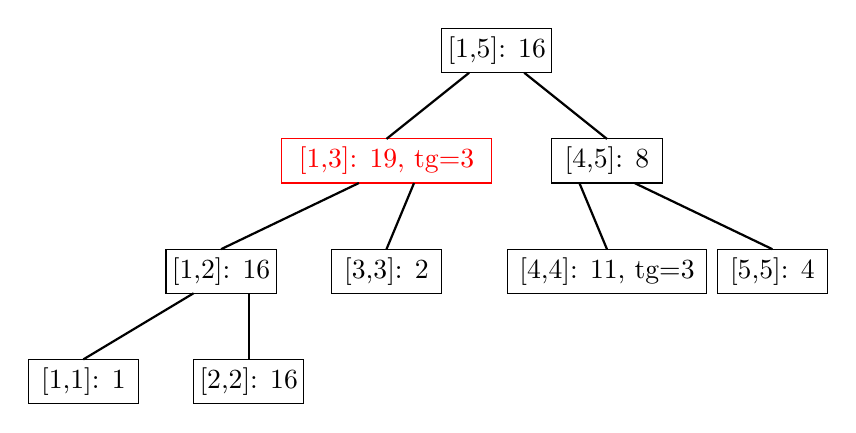
\begin{tikzpicture}[scale=0.7]
          \draw [black] (-1,7.9) rectangle (1,7.1) node [black, midway] {[1,5]: 16}; % Draws a rectangle

          \draw [red] (-3.9,5.9) rectangle (-0.1,5.1) node [red,midway] {[1,3]: 19, tg=3}; % Draws a rectangle
          \draw [black] (1,5.9) rectangle (3,5.1) node [black,midway] {[4,5]: 8}; % Draws a rectangle

          \draw [black] (-6,3.9) rectangle (-4,3.1) node [black,midway] {[1,2]: 16}; % Draws a rectangle
          \draw [black] (-3,3.9) rectangle (-1,3.1) node [black,midway] {[3,3]: 2}; % Draws a rectangle
          \draw [black] (0.2,3.9) rectangle (3.8,3.1) node [black,midway] {[4,4]: 11, tg=3}; % Draws a rectangle
          \draw [black] (4,3.9) rectangle (6,3.1) node [black,midway] {[5,5]: 4}; % Draws a rectangle

          \draw [black] (-8.5,1.9) rectangle (-6.5,1.1) node [black,midway] {[1,1]: 1}; % Draws a rectangle
          \draw [black] (-5.5,1.9) rectangle (-3.5,1.1) node [black,midway] {[2,2]: 16}; % Draws a rectangle

          \draw [thick] (-0.5,7.1) to (-2,5.9);
          \draw [thick] (0.5,7.1) to (2,5.9);

          \draw [thick] (-2.5,5.1) to (-5,3.9);
          \draw [thick] (-1.5,5.1) to (-2,3.9);

          \draw [thick] (1.5,5.1) to (2,3.9);
          \draw [thick] (2.5,5.1) to (5,3.9);

          \draw [thick] (-5.5,3.1) to (-7.5,1.9);
          \draw [thick] (-4.5,3.1) to (-4.5,1.9);
          % \draw [thick] (-2,2) % Draws a line
          % to [out=10,in=190] (2,2)
          % to [out=10,in=90] (6,0) 
          % to [out=-90,in=30] (-2,-2);    
        \end{tikzpicture}
      \end{figure}
  \end{itemize}
\end{frame}

\begin{frame}[fragile]{\btitle{懶人標記}}
  \begin{itemize}
    \item $a = [1, 16, 2, 8, 4]$,並把 $[1, 4]$ 加上 $3$,詢問 $[3, 3]$ 的最大值
    \item 把 tag 往下推?其實就是告訴左右孩子底下所有元素必須要加上 $3$
      \begin{figure}
        \begin{tikzpicture}[scale=0.7]
          \draw [black] (-1,7.9) rectangle (1,7.1) node [black, midway] {[1,5]: 16}; % Draws a rectangle

          \draw [red] (-3.9,5.9) rectangle (-0.1,5.1) node [red,midway] {[1,3]: 19, tg=3}; % Draws a rectangle
          \draw [black] (1,5.9) rectangle (3,5.1) node [black,midway] {[4,5]: 8}; % Draws a rectangle

          \draw [blue] (-6,3.9) rectangle (-4,3.1) node [blue,midway] {[1,2]: 16}; % Draws a rectangle
          \draw [blue] (-3,3.9) rectangle (-1,3.1) node [blue,midway] {[3,3]: 2}; % Draws a rectangle
          \draw [black] (0.2,3.9) rectangle (3.8,3.1) node [black,midway] {[4,4]: 11, tg=3}; % Draws a rectangle
          \draw [black] (4,3.9) rectangle (6,3.1) node [black,midway] {[5,5]: 4}; % Draws a rectangle

          \draw [black] (-8.5,1.9) rectangle (-6.5,1.1) node [black,midway] {[1,1]: 1}; % Draws a rectangle
          \draw [black] (-5.5,1.9) rectangle (-3.5,1.1) node [black,midway] {[2,2]: 16}; % Draws a rectangle

          \draw [thick] (-0.5,7.1) to (-2,5.9);
          \draw [thick] (0.5,7.1) to (2,5.9);

          \draw [red, arrows=-{Latex[length=3mm]}] (-2.5,5.1) -- (-5,3.9);
          \draw [red, arrows=-{Latex[length=3mm]}] (-1.5,5.1) -- (-2,3.9);

          \draw [thick] (1.5,5.1) to (2,3.9);
          \draw [thick] (2.5,5.1) to (5,3.9);

          \draw [thick] (-5.5,3.1) to (-7.5,1.9);
          \draw [thick] (-4.5,3.1) to (-4.5,1.9);
          % \draw [thick] (-2,2) % Draws a line
          % to [out=10,in=190] (2,2)
          % to [out=10,in=90] (6,0) 
          % to [out=-90,in=30] (-2,-2);    
        \end{tikzpicture}
      \end{figure}
  \end{itemize}
\end{frame}

\begin{frame}[fragile]{\btitle{懶人標記}}
  \begin{itemize}
    \item $a = [1, 16, 2, 8, 4]$,並把 $[1, 4]$ 加上 $3$,詢問 $[3, 3]$ 的最大值
    \item 把 tag 資訊丟給左右子樹,並且更新左右子樹的答案
      \begin{figure}
        \begin{tikzpicture}[scale=0.7]
          \draw [black] (-1,7.9) rectangle (1,7.1) node [black, midway] {[1,5]: 16}; % Draws a rectangle

          \draw [red] (-3.9,5.9) rectangle (-0.1,5.1) node [red,midway] {[1,3]: 19, tg=3}; % Draws a rectangle
          \draw [black] (1,5.9) rectangle (3,5.1) node [black,midway] {[4,5]: 8}; % Draws a rectangle

          \draw [blue] (-6.6,3.9) rectangle (-3.2,3.1) node [blue,midway] {[1,2]:19,tg=3}; % Draws a rectangle
          \draw [blue] (-3.1,3.9) rectangle (-0.1,3.1) node [blue,midway] {[3,3]:5,tg=3}; % Draws a rectangle
          \draw [black] (0.2,3.9) rectangle (3.8,3.1) node [black,midway] {[4,4]: 11, tg=3}; % Draws a rectangle
          \draw [black] (4,3.9) rectangle (6,3.1) node [black,midway] {[5,5]: 4}; % Draws a rectangle

          \draw [black] (-8.5,1.9) rectangle (-6.5,1.1) node [black,midway] {[1,1]: 1}; % Draws a rectangle
          \draw [black] (-5.5,1.9) rectangle (-3.5,1.1) node [black,midway] {[2,2]: 16}; % Draws a rectangle

          \draw [thick] (-0.5,7.1) to (-2,5.9);
          \draw [thick] (0.5,7.1) to (2,5.9);

          \draw [red, arrows=-{Latex[length=3mm]}] (-2.5,5.1) -- (-5,3.9);
          \draw [red, arrows=-{Latex[length=3mm]}] (-1.5,5.1) -- (-2,3.9);

          \draw [thick] (1.5,5.1) to (2,3.9);
          \draw [thick] (2.5,5.1) to (5,3.9);

          \draw [thick] (-5.5,3.1) to (-7.5,1.9);
          \draw [thick] (-4.5,3.1) to (-4.5,1.9);
          % \draw [thick] (-2,2) % Draws a line
          % to [out=10,in=190] (2,2)
          % to [out=10,in=90] (6,0) 
          % to [out=-90,in=30] (-2,-2);    
        \end{tikzpicture}
      \end{figure}
  \end{itemize}
\end{frame}

\begin{frame}[fragile]{\btitle{懶人標記}}
  \begin{itemize}
    \item $a = [1, 16, 2, 8, 4]$,並把 $[1, 4]$ 加上 $3$,詢問 $[3, 3]$ 的最大值
    \item 原本的 tag 功成身退!
      \begin{figure}
        \begin{tikzpicture}[scale=0.7]
          \draw [black] (-1,7.9) rectangle (1,7.1) node [black, midway] {[1,5]: 16}; % Draws a rectangle

          \draw [red] (-3.9,5.9) rectangle (-0.1,5.1) node [red,midway] {[1,3]: 19}; % Draws a rectangle
          \draw [black] (1,5.9) rectangle (3,5.1) node [black,midway] {[4,5]: 8}; % Draws a rectangle

          \draw [blue] (-6.6,3.9) rectangle (-3.2,3.1) node [blue,midway] {[1,2]:19,tg=3}; % Draws a rectangle
          \draw [blue] (-3.1,3.9) rectangle (-0.1,3.1) node [blue,midway] {[3,3]:5,tg=3}; % Draws a rectangle
          \draw [black] (0.2,3.9) rectangle (3.8,3.1) node [black,midway] {[4,4]: 11, tg=3}; % Draws a rectangle
          \draw [black] (4,3.9) rectangle (6,3.1) node [black,midway] {[5,5]: 4}; % Draws a rectangle

          \draw [black] (-8.5,1.9) rectangle (-6.5,1.1) node [black,midway] {[1,1]: 1}; % Draws a rectangle
          \draw [black] (-5.5,1.9) rectangle (-3.5,1.1) node [black,midway] {[2,2]: 16}; % Draws a rectangle

          \draw [thick] (-0.5,7.1) to (-2,5.9);
          \draw [thick] (0.5,7.1) to (2,5.9);

          \draw [red, arrows=-{Latex[length=3mm]}] (-2.5,5.1) -- (-5,3.9);
          \draw [red, arrows=-{Latex[length=3mm]}] (-1.5,5.1) -- (-2,3.9);

          \draw [thick] (1.5,5.1) to (2,3.9);
          \draw [thick] (2.5,5.1) to (5,3.9);

          \draw [thick] (-5.5,3.1) to (-7.5,1.9);
          \draw [thick] (-4.5,3.1) to (-4.5,1.9);
          % \draw [thick] (-2,2) % Draws a line
          % to [out=10,in=190] (2,2)
          % to [out=10,in=90] (6,0) 
          % to [out=-90,in=30] (-2,-2);    
        \end{tikzpicture}
      \end{figure}
  \end{itemize}
\end{frame}

\begin{frame}[fragile]{\btitle{懶人標記}}
  \begin{itemize}
    \item 具體來說,之後某次區間修改或查詢而\textbf{造訪到某個節點時,我們才將這個節點的「標記」往下推},把標記的資訊傳給小孩
    \item 推標記的複雜度是 $O(1)$,不影響原本的複雜度!
    \item 因為是只在必要的時候更新標記,因此這個技巧又被稱為\textbf{懶人標記}
    \item 我們常把推標記的函數叫做 \texttt{push();}
    \item 直接來看程式碼吧~
  \end{itemize}
\end{frame}

\begin{frame}[fragile]{\btitle{懶人標記}}
  \begin{minted}[breaklines]{cpp}
    struct Node {
      Node *lc, *rc;
      int mx, tag; // tag 左右子樹整個子樹需要加上的數值
      void pull() { mx = max(lc->mx, rc->mx); }
    } *root = nullptr;
  \end{minted}
\end{frame}

\begin{frame}[fragile]{\btitle{懶人標記}}
  \begin{minted}[breaklines]{cpp}
    void push(Node *nd, int l, int r) {
      // 把 nd 的 tag 往左右子樹推
      if (l == r) nd->tag = 0;
      if (!nd->tag) return;
      nd->lc->tag += nd->tag; // 左子樹的 tag 跟 nd 的 tag 合併,這題 tag 是加上數值,因此直接加起來就可以
      nd->lc->mx  += nd->tag; // 左子樹的最大值加上 nd 的 tag
      nd->rc->tag += nd->tag;
      nd->rc->mx  += nd->tag;
      nd->tag = 0; // 清空 tag
    }
  \end{minted}
\end{frame}

\begin{frame}[fragile]{\btitle{懶人標記}}
  \begin{minted}[breaklines]{cpp}
    void modify(Node *nd, int ql, int qr, int d, int l, int r) {
      if (r < ql || l > qr)
        return;
      if (ql <= l && r <= qr) {
        nd->mx += d;  // 當前前點的所有數字加上 d,最大值也需要加上 d
        nd->tag += d; // 告訴左右子樹,最大值需要加上 d
        return;
      }
      push(nd, l, r); // 需要拜訪子樹的時候,把當前點的 tag 往下推
      int m = (l + r) / 2;
      modify(nd->lc, ql, qr, d, l, m);
      modify(nd->rc, ql, qr, d, m + 1, r);
      nd->pull();
    }
  \end{minted}
\end{frame}

\begin{frame}[fragile]{\btitle{懶人標記}}
  \begin{minted}[breaklines]{cpp}
    int query(Node *nd, int ql, int qr, int l, int r) {
      if (r < ql || l > qr)
        return 0;
      if (ql <= l && r <= qr)
        return nd->mx;
      push(nd, l, r); // 需要拜訪子樹的時候,把當前點的 tag 往下推
      int m = (l + r) / 2;
      return max(query(nd->lc, ql, qr, l, m), query(nd->rc, ql, qr, m + 1, r));
    }
  \end{minted}
\end{frame}

\begin{frame}[fragile]{\btitle{懶人標記}}
  \begin{itemize}
    \item 使用時機?
    \item 標記必須要可以合併、並且能夠快速的由「標記」所儲存的資訊推出這個節點的資訊應該被修改成什麼
    \item 有的時候順序很重要!
    \item 常見出現時機:區間加值區間求和、區間加值區間取 max、區間加值區間乘值區間求和......等等
    \item 不知道大家有沒有發現,\texttt{push()} 跟 \texttt{pull()} 好像會成對出現!
    \item 課外閱讀:有一種標記的方式叫「永久化標記」,這種標記就會直接把懶標固定在節點上,但詢問的時候就要多處理一些東西
  \end{itemize}
\end{frame}

\begin{frame}[fragile]{\btitle{copy on write 線段樹}}
  \begin{itemize}
    \item 又稱動態開點線段樹
    \item 需要使用的時候再把節點開出來!
    \item 直接來看例題:
    \begin{problem}[二維區間求和]
      給一 $N \times N(N \leq 10^9)$ 二維平面初始所有值都是零,$Q(Q \leq 10^5)$ 筆操作,操作包含兩種:
      \begin{itemize}
        \item \texttt{add x y d}: 將座標 $(x,y)$ 的元素加上 d
        \item \texttt{query x1 y1 x2 y2}: 詢問所有 $(x,y)$ 滿足 $x1 \leq x \leq x2$ 且 $y1 \leq y \leq y2$ 的總和。
      \end{itemize}
    \end{problem}
  \end{itemize}
\end{frame}

\begin{frame}[fragile]{\btitle{copy on write 線段樹}}
  \begin{itemize}
    \item 從題目的操作可以得知,最多只會有 $10^5$ 個座標有值
    \item 若是定義在一維座標上,我們可以利用\textbf{離散化}的技巧依然用我們前面介紹的線段樹解決
  \end{itemize}
\end{frame}

\begin{frame}[fragile]{\btitle{copy on write 線段樹}}
  \begin{itemize}    
    \item 然而,我們現在要處理的是二維座標
    \item 試著用線段樹套線段樹的方式吧!
    \item 等等,什麼是線段樹套線段樹?
  \end{itemize}
\end{frame}

\begin{frame}[fragile]{\btitle{copy on write 線段樹}}
  \begin{itemize}    
    \item 對 $x$ 軸開一個線段樹,$x$ 軸相關的節點的內容是對 $y$ 軸的線段樹!
      \begin{figure}
        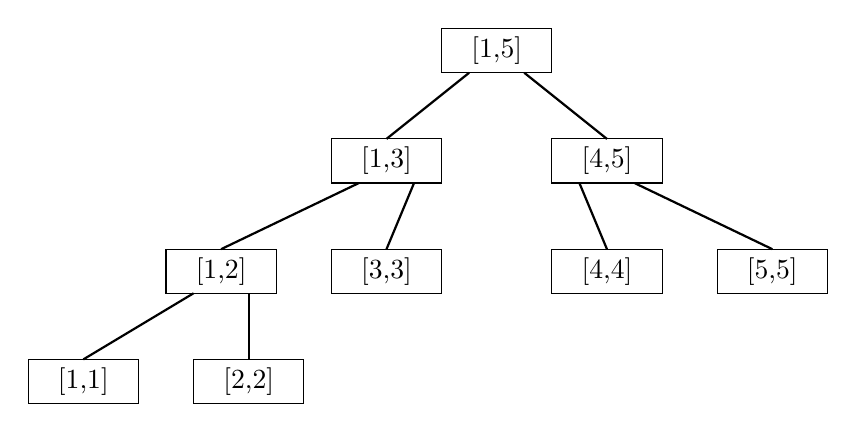
\begin{tikzpicture}[scale=0.7]
          \draw [black] (-1,7.9) rectangle (1,7.1) node [black, midway] {[1,5]}; % Draws a rectangle

          \draw [black] (-3,5.9) rectangle (-1,5.1) node [black,midway] {[1,3]}; % Draws a rectangle
          \draw [black] (1,5.9) rectangle (3,5.1) node [black,midway] {[4,5]}; % Draws a rectangle

          \draw [black] (-6,3.9) rectangle (-4,3.1) node [black,midway] {[1,2]}; % Draws a rectangle
          \draw [black] (-3,3.9) rectangle (-1,3.1) node [black,midway] {[3,3]}; % Draws a rectangle
          \draw [black] (1,3.9) rectangle (3,3.1) node [black,midway] {[4,4]}; % Draws a rectangle
          \draw [black] (4,3.9) rectangle (6,3.1) node [black,midway] {[5,5]}; % Draws a rectangle

          \draw [black] (-8.5,1.9) rectangle (-6.5,1.1) node [black,midway] {[1,1]}; % Draws a rectangle
          \draw [black] (-5.5,1.9) rectangle (-3.5,1.1) node [black,midway] {[2,2]}; % Draws a rectangle

          \draw [thick] (-0.5,7.1) to (-2,5.9);
          \draw [thick] (0.5,7.1) to (2,5.9);

          \draw [thick] (-2.5,5.1) to (-5,3.9);
          \draw [thick] (-1.5,5.1) to (-2,3.9);

          \draw [thick] (1.5,5.1) to (2,3.9);
          \draw [thick] (2.5,5.1) to (5,3.9);

          \draw [thick] (-5.5,3.1) to (-7.5,1.9);
          \draw [thick] (-4.5,3.1) to (-4.5,1.9);
          % \draw [thick] (-2,2) % Draws a line
          % to [out=10,in=190] (2,2)
          % to [out=10,in=90] (6,0) 
          % to [out=-90,in=30] (-2,-2);
        \end{tikzpicture}
      \end{figure}
    \item 比如說,$[1, 3]$ 這個節點存一個 $y$ 軸資訊的線段樹,$y$ 軸線段樹的 $[4, 5]$ 就是存 $[1..3, 4..5]$ 的總和!
  \end{itemize}
\end{frame}

\begin{frame}[fragile]{\btitle{copy on write 線段樹}}
  \begin{itemize}    
    \item 雖然做完離散化,還是 $O(Q^2)$ 的空間
    \item 但,最多只有 $Q$ 個座標有值,因此,最多只有 $O(Q \lg^2 N)$ 個節點有值!只要能只記錄這些節點便勝利了
    \begin{itemize}
      \item 在 $x$ 軸的世界中會經過 $O(\log N)$ 個節點
      \item 每個節點的線段樹需要經過 $O(\log N)$ 個 $y$ 軸節點
    \end{itemize}
    \item 來看 code 吧!
  \end{itemize}
\end{frame}

\begin{frame}[fragile]{\btitle{copy on write 線段樹}}
  \begin{minted}[breaklines]{cpp}
    struct Node2 { // 第二個維度的線段樹節點
      int val;
      Node2 *lc, *rc;
      Node2() {
        val = 0;
        lc = rc = NULL;
      }
    };
    struct Node1 { // 第一個維度的線段樹節點
      Node1 *lc, *rc;
      Node2 *c;
      Node1() {
        c = NULL;
        lc = rc = NULL;
      }
    };
  \end{minted}
\end{frame}

\begin{frame}[fragile]{\btitle{copy on write 線段樹}}
  \begin{minted}[breaklines]{cpp}
    int Val2(Node2 *node) { return node ? node->val : 0; }
    void pull2(Node2 *node) { node->val = Val2(node->lc) + Val2(node->rc); }
  \end{minted}
\end{frame}

\begin{frame}[fragile]{\btitle{copy on write 線段樹}}
  \begin{minted}[breaklines]{cpp}
    void modify2(Node2 *node, int Y1, int Y2, int qy, int d) {
      if (Y1 == Y2) {
        node->val += d;
        return;
      }
      int mid = (Y1 + Y2) >> 1;
      if (qy <= mid) {
        if (!node->lc) node->lc = new Node2(); // 有需要再開新的 y 軸點
        modify2(node->lc, Y1, mid, qy, d);
      } else {
        if (!node->rc) node->rc = new Node2();
        modify2(node->rc, mid + 1, Y2, qy, d);
      }
      pull2(node);
    }
  \end{minted}
\end{frame}

\begin{frame}[fragile]{\btitle{copy on write 線段樹}}
  \begin{minted}[breaklines]{cpp}
    void modify1(Node1 *node, int X1, int X2, int qx, int qy, int d) {
      if (!node->c) node->c = new Node2(); // 有需要再開新的 y 軸點
      modify2(node->c, 1, n, qy, d);
      if (X1 == X2) {
        return;
      }
      int mid = (X1 + X2) >> 1;
      if (qx <= mid) {
        if (!node->lc) node->lc = new Node1(); // 有需要再開新的 x 軸點
        modify1(node->lc, X1, mid, qx, qy, d);
      } else {
        if (!node->rc) node->rc = new Node1();
        modify1(node->rc, mid + 1, X2, qx, qy, d);
      }
    }
  \end{minted}
\end{frame}

\begin{frame}[fragile]{\btitle{copy on write 線段樹}}
  \begin{minted}[breaklines]{cpp}
    int query2(Node2 *node, int Y1, int Y2, int qy1, int qy2) {
      if (qy1 > Y2 || qy2 < Y1)
        return 0;
      if (!node)
        return 0; // no data!
      if (qy1 <= Y1 && Y2 <= qy2)
        return node->val;
      int mid = (Y1 + Y2) >> 1;
      return query2(node->lc, Y1, mid, qy1, qy2) +
             query2(node->rc, mid + 1, Y2, qy1, qy2);
    }
  \end{minted}
\end{frame}

\begin{frame}[fragile]{\btitle{copy on write 線段樹}}
  \begin{minted}[breaklines]{cpp}
    int query1(Node1 *node, int X1, int X2, int qx1, int qx2, int qy1, int qy2) {
      if (qx1 > X2 || qx2 < X1)
        return 0;
      if (!node)
        return 0; // no data!
      if (qx1 <= X1 && X2 <= qx2)
        return query2(node->c, 1, n, qy1, qy2);
      int mid = (X1 + X2) >> 1;
      return query1(node->lc, X1, mid, qx1, qx2, qy1, qy2) +
             query1(node->rc, mid + 1, X2, qx1, qx2, qy1, qy2);
    }
  \end{minted}
\end{frame}

\begin{frame}[fragile]{\btitle{持久化線段樹}}
  \begin{itemize}
    \item 修改後依舊保有歷史版本的資料結構
    \item 直接來看例題:
    \begin{problem}[歷史版本和]
      給定一個長度 $N$ 的序列以及 $M$ 個單點修改,接下來有 $Q$ 次詢問,每次詢問會問你在第 $m$ 次修改後,區間 $[l, r]$ 的總和是多少。
      強制在線。
      
      \begin{itemize}
          \item
              $N, Q \leq 10^5$
      \end{itemize}
    \end{problem}
  \end{itemize}
\end{frame}

\begin{frame}[fragile]{\btitle{持久化線段樹}}
  \begin{itemize}
    \item 我會!
    \item 每個版本各開一個線段樹就好啦~
    \item 總共需要 $O(N)$ 個版本,每個版本 $O(N)$ 個點,總共 $O(N^2)$ 個點,TLE!
    \item 怎麼辦 OuO
  \end{itemize}
\end{frame}

\begin{frame}[fragile]{\btitle{持久化線段樹}}
  \begin{itemize}
    \item 努力觀察一下:每次修改都只會動到 $O(\log N)$ 個節點
      \begin{itemize}
        \item 這些節點其實就是單點修改碰到的那些點
      \end{itemize}
    \item 那麼我們為何不能用 $O(\log N)$ 的空間來儲存兩個版本之間的差距呢?
  \end{itemize}
\end{frame}

\begin{frame}[fragile]{\btitle{持久化線段樹}}
  \begin{itemize}
    \item 努力觀察一下:每次修改都只會動到 $O(\log N)$ 個節點
    \item 那麼我們為何不能用 $O(\log N)$ 的空間來儲存兩個版本之間的差距呢?
    \item 具體來說,我們每次想要更新一個節點的值時,會開出一個新節點儲存修改之後的資訊(不要看下面那張圖的 $e$ 點)
  \end{itemize}
  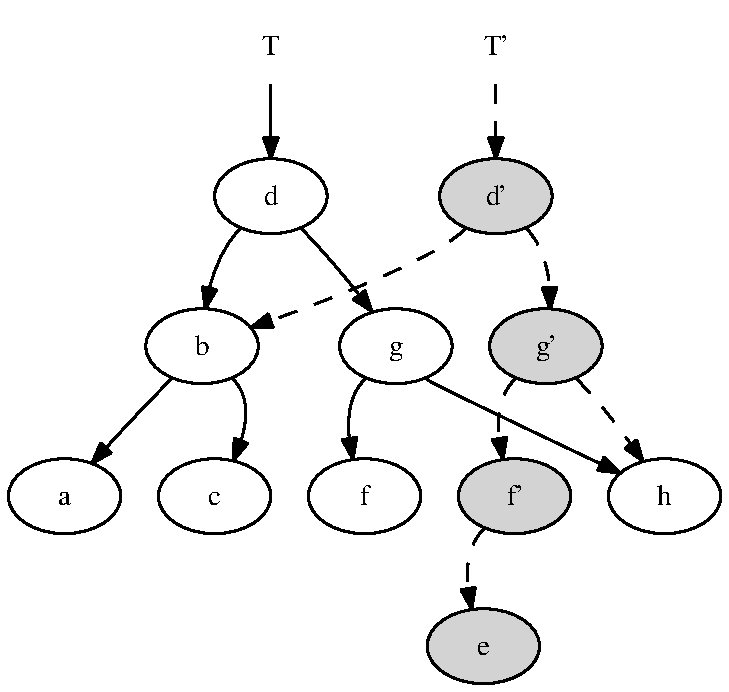
\includegraphics[height=4.5cm]{figures/persistent-tree.pdf}
\end{frame}

\begin{frame}[fragile]{\btitle{持久化線段樹}}
  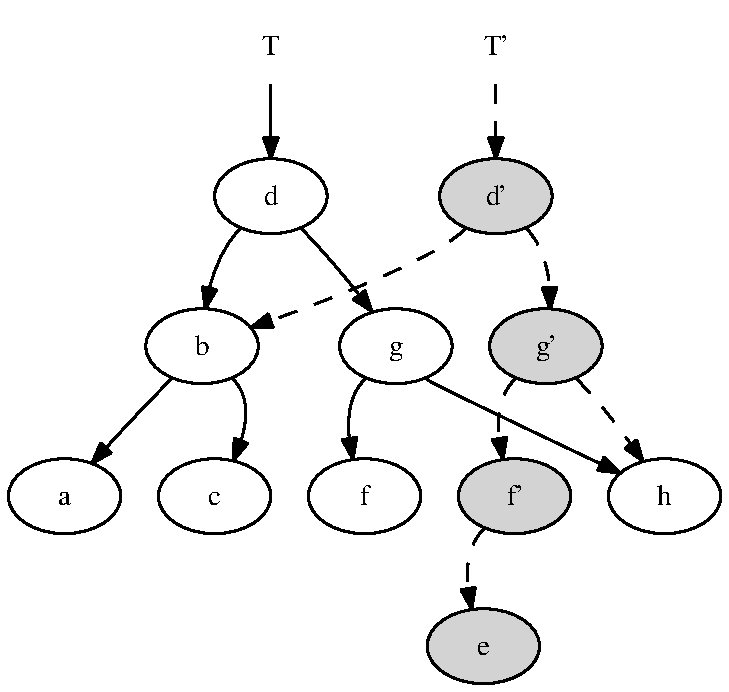
\includegraphics[height=4.5cm]{figures/persistent-tree.pdf}
  \begin{itemize}
    \item 所以,每當需要一個新的版本的時候
    \item 先把舊版本根節點重新複製一遍到新版本的根節點上
    \item 每當要進入某個點修改時,先把該節點複製一份到新版本上
    \item 遞迴修改
    \item 修改結束後,因為新節點的子樹有變動,呼叫新節點的 \texttt{pull()}
  \end{itemize}
\end{frame}

\begin{frame}[fragile]{\btitle{持久化線段樹}}
  \begin{minted}[breaklines]{cpp}
    // get a copy of node
    Node *getNode(Node *node) {
      Node *tnode = new Node();
      tnode->val = node->val;
      tnode->lc = node->lc;
      tnode->rc = node->rc;
      return tnode;
    }
  \end{minted}
\end{frame}

\begin{frame}[fragile]{\btitle{持久化線段樹}}
  \begin{minted}[breaklines]{cpp}
    void modify(Node *node, Node *newNode, int L, int R, int i, int d) {
      if (L == R) {
        newNode->val += d;
        return;
      }
      int mid = (L + R) >> 1;
      if (i <= mid) {
        newNode->lc = getNode(node->lc);
        modify(node->lc, newNode->lc, L, mid, i, d);
      } else {
        newNode->rc = getNode(node->rc);
        modify(node->rc, newNode->rc, mid + 1, R, i, d);
      }
      newNode->pull();
    }
  \end{minted}
\end{frame}

\begin{frame}[fragile]{\btitle{持久化線段樹}}
  \begin{itemize}
    \item 很常運用在序列上!
    \item 常見建立的版本時機是:給定一個長度為 $N$ 的序列,建立 $N$ 個版本,第 $i$ 個版本維護第 $i$ 個位置的前綴(或者是後綴)的資訊
  \end{itemize}
\end{frame}

\begin{frame}[fragile]{\btitle{STL in 線段樹}}
  \begin{itemize}
    \item 線段樹的節點可以塞各式各樣的東西喔!
    \begin{problem}[二維區間求和]
      有 $n$ 個目標物,每個目標物都是一個水平線段 $[s, t]$ 或是只含一點($s = t$ 的情形),並且有各自的分數 $w$,所有目標物的高度($y$ 值)均大於 $0$ 且互不相同(輸入按照 $y$ 座標由大到小排序)。
      現在依序發射了 $m$ 發砲彈,第 $i$ 次會從 $x$ 軸上的整數點 $x_i$ 往上垂直發射砲彈,路線上第一個碰到的目標物就是擊中的目標,射中目標後砲彈與目標物一起消失,不會穿透。如果沒有擊中任何目標物,則該次射擊分數為 0。請輸出每次有擊中的目標物的分數總和。
      \begin{itemize}
        \item $n, m \leq 5 \times 10^5$
        \item $s,t,x_i \leq 10^6$
      \end{itemize}
    \end{problem}
  \end{itemize}
\end{frame}

\begin{frame}[fragile]{\btitle{STL in 線段樹}}
  \begin{itemize}
    \item 在線段樹的每個節點當中,我們可以儲存一個 set
    \item set 裡面放一些完全包含這個節點對應的區間的水平線段
    \item 我們可以做 $n$ 次的區間修改,在對應的節點裡面的 set 插入這個水平線段的 $y$ 座標
    \item 對於每次的單點詢問,我們查看對應的葉節點到根的這條路徑上, $y$ 座標最小的水平線段是哪一個
    \item 當知道哪個水平線段要被刪除之後,可以做一次區間修改,並且在對應的節點裡面的 set 刪除這個水平線段的 $y$ 座標
    \item 因為每次都會造訪 $O(\log n)$ 個節點,而 std::set 插入、刪除的複雜度都是 $O(\log n)$,因此總共的複雜度會是 $((n+m)\log ^2 n)$,空間複雜度則是 $O(n\log n)$
  \end{itemize}
\end{frame}

\begin{frame}[fragile]{\btitle{STL in 線段樹}}
  \begin{itemize}
    \item 事實上我們可以用一個 std::vector(或是 stack)來維護這樣的插入與刪除,因為所有刪除操作都在插入之後,如此時間複雜度可以減少一個 $\log$
    \item 注意 STL 的 stack 內部預設是 deque,而空的 deque 佔的空間很多,因此在這種嵌套的資料結構特別要小心
  \end{itemize}
\end{frame}

\begin{frame}[fragile]{\btitle{區間查詢與修改的對偶}}
  \begin{itemize}
    \item 直接來看例題!
    \begin{problem}[區間取 max、單點查詢]
      有一長度為 $N$ 的序列 $a_1,a_2,\dots,a_N$,一開始全部為 $0$。接下來有 $M$ 個操作,每個操作形如 $l, r, v$ ,表示對於所有 $l \leq i \leq r$,$a_i := \max(a_i, v)$。
      請你分別輸出 $a_1,a_2,\dots, a_N$ 最後的值是多少。

      \begin{itemize}
          \item
              $N \leq 2\times 10^5$
          \item
              $M \leq 5\times 10^6$
      \end{itemize}
    \end{problem}
  \end{itemize}
\end{frame}

\begin{frame}[fragile]{\btitle{區間查詢與修改的對偶}}
  \begin{itemize}
    \item 相信在前面學過懶人標記後,大家已經知道如何用線段樹與懶人標記解決這個問題了
    \item 然而這樣做的複雜度是 $O(N+M\log N)$,很有可能無法在時限內通過
    \item 為什麼呢?因為詢問的數量太多了
    \item 但相對的,\textbf{修改沒那麼多},並且\textbf{我們可以一次處理所有修改}
    \item 有什麼資料結構是支援快速查詢,且可以利用離線的性質呢?
    \item Sparse Table!
  \end{itemize}
\end{frame}

\begin{frame}[fragile]{\btitle{區間查詢與修改的對偶}}
  \begin{itemize}
    \item 在 Sparse Table 中是把一個區間查詢拆成兩個部份重疊的區間查詢,並且兩個區間的長度為 2 的冪次
    \item 那麼我們也可以把區間修改拆成兩個長度為 2 的冪次的區間,並紀錄所有 $g(i, j)$ 表示 $[i, i+2^j)$ 整個區間要跟多少取 max
    \item 最後再一次花 $O(N\log N)$ DP 便能得到每個單獨的位置是多少
      \begin{itemize}
        \item 類似 sparse table 預處理的方式
        \item 只是這次是從上面往下推(sparse table 預處理是下面往上推)
      \end{itemize}
    \item 因此總複雜度為 $O(N\log N + M)$,空間複雜度是 $O(N\log N)$
  \end{itemize}
\end{frame}

\begin{frame}[fragile]{\btitle{區間查詢與修改的對偶}}
  \begin{minted}[breaklines]{cpp}
    int st[maxlg][maxn];
    void chmax(int l, int r, int val) {
      // for i \in [l, r), a[i] = max(a[i], val)
      int lg = __lg(r - l);
      int len = 1 << lg;
      st[lg][l] = max(st[lg][l], val);
      st[lg][r - len] = max(st[lg][r - len], val);
    }
  \end{minted}
\end{frame}

\begin{frame}[fragile]{\btitle{區間查詢與修改的對偶}}
  \begin{minted}[breaklines]{cpp}
    void dp(int n) {
      for (int l = maxlg - 2; l >= 0; l--) {
        int len = 1 << l;
        for (int i = 0; i < n; i++) {
          st[l][i] = max(st[l][i], st[l + 1][i]);
          if (i + len < n)
            st[l][i + len] = max(st[l][i + len], st[l + 1][i]);
        }
      }
      // ans is st[0][i]
    }
  \end{minted}
\end{frame}

\begin{frame}[fragile]{\btitle{區間查詢與修改的對偶}}
  \begin{itemize}
    \item 網路上有一個類似的技巧被稱為 Dual Segment Tree,但比較侷限在線段樹而沒有其他推廣
    \item 事實上這個技巧除了 Sparse Table 外,分塊、樹上倍增法、線段樹都可以用到
    \item 值得注意的是線段樹一次 push 所有節點的懶標只需要 $O(N)$
      \begin{itemize}
        \item DFS 一次整棵樹就可以了!
      \end{itemize}
  \end{itemize}
\end{frame}

\begin{frame}[fragile]{\btitle{線段樹上的均攤}}
  \begin{itemize}
    \item 直接來看例題!
    \begin{problem}[區間取 max、單點查詢]
      給定一個長度 $N$ 的序列 $a_1,\dots,a_N$,接下來有 $Q$ 個操作:
      \begin{itemize}
          \item \(\texttt{A x v}\) 將 $a_x$ 改為 $v$。
          \item \(\texttt{D l r k}\) 對於所有 $l\leq i\leq r$,將 $a_i$ 改為 $\lfloor \frac{a_i}{k} \rfloor$。
          \item \(\texttt{S l r}\) 查詢區間 $[l, r]$ 的總和。
      \end{itemize}
      輸入的所有數字均為正整數。

      \begin{itemize}
          \item
              $N, Q \leq 10^5$
          \item
              $1 \leq a_i, v, k \leq 10^9$
      \end{itemize}
    \end{problem}
  \end{itemize}
\end{frame}

\begin{frame}[fragile]{\btitle{線段樹上的均攤}}
  \begin{itemize}
    \item 本題出現了一個非常神秘的操作:區間除法取下高斯
    \item 我們無法快速由分母推出整個區間的總和如何變化,要怎麼處理這樣的問題呢?
    \item 不是整個區間都是 $0$,就暴力 DFS 下去!
    \item 這樣是好的嗎...... (?)
    \item 亂寫一通就發現 AC 了,怎麼會這樣!
  \end{itemize}
\end{frame}

\begin{frame}[fragile]{\btitle{線段樹上的均攤}}
  \begin{itemize}
    \item 可以發現,每個數字被除了 $O(\log C)$ 次之後就會變成 $0$(當然,不包含 $k=1$ 的情況)
    \item 而每個數字每除一次又最多只會讓時間增加樹高的量級
    \item 至於單點修改也只會讓除的次數增加 $\log C$ 次
    \item 因此,總複雜度便是 $O((N+Q)\log N \log C)$
    \item 除了除法之外,區間開根號、區間取 $\log$ 都可以用類似的技巧喔!
  \end{itemize}
\end{frame}

\begin{frame}[fragile]{\btitle{搭配離線演算法}}
  \begin{itemize}
    \item 「離線回答的精髓」:可以事前知道所有詢問的所有參數,並且可以不按順序回答每個詢問
    \item 什麼意思?來看前面持久化線段樹例題的離線版本
    \item
      \begin{problem}[歷史版本和 -- offline]
        給定一個長度 $N$ 的序列以及 $M$ 個單點修改,接下來有 $Q$ 次詢問,每次詢問會問你在第 $m$ 次修改後,區間 $[l, r]$ 的總和是多少。
        
        \begin{itemize}
            \item
                $N, Q \leq 10^5$
        \end{itemize}
      \end{problem}
    \item 為什麼我不要乾脆一邊做修改、等到剛好第 $m$ 次修改之後再回答詢問就好了
    \item 而這個就是「離線回答的精髓」:可以事前知道所有詢問的所有參數,並且可以不按順序回答每個詢問
  \end{itemize}
\end{frame}

\begin{frame}[fragile]{\btitle{搭配離線演算法}}
  \begin{itemize}    
    \item 離線演算法大致上的套路都是把詢問和修改(原本的序列也可以當成是某種修改)一起按照某種順序排序
    \item 接著一邊處理修改一邊處理詢問
    \item 並把所有詢問的答案存下來後一次回答全部
    \item 事實上,許多問題「在線回答」與「離線回答」的難度相差很多,也有很多知名的演算法必須在離線的問題才能使用
    \item 來看例題吧!
  \end{itemize}
\end{frame}

\begin{frame}[fragile]{\btitle{搭配離線演算法}}
  \begin{itemize}
    \item 
      \begin{problem}[區間 mex]
        給定一個序列 $a_1,a_2,\dots,a_N$,接下來有 $Q$ 個詢問,每次會給定 $l, r$,請你回答 $\operatorname{mex}(a_l,a_{l+1},\dots,a_r)$。
        其中 $\operatorname{mex}$ 的定義是一個集合中最小未出現的非負整數。

        \begin{itemize}
            \item
                $N, Q \leq 2\times 10^5$
        \end{itemize}

        比如說,$\operatorname{mex}(1, 3) = 0$, $\operatorname{mex}(0, 1, 3) = 2$
      \end{problem}
    \item 題外話:這題可以用莫隊 + 值域分塊在 $O((N + Q)\sqrt{N})$ 做掉,不過不在這堂課的討論範疇(偷偷工商,可以看資芽 2021 年根號 inclass 的投影片喔)
    \item 好像不太清楚 \texttt{pull()} 要怎麼寫耶,怎麼辦?
    \item 先來考慮一個簡單一點的版本!
  \end{itemize}
\end{frame}

\begin{frame}[fragile]{\btitle{搭配離線演算法}}
  \begin{itemize}
    \item 
      \begin{problem}[區間 mex --- 簡化版]
        給定一個序列 $a_1,a_2,\dots,a_N$,接下來有 $Q$ 個詢問,每次會給定 $r$,請你回答 $\operatorname{mex}(a_1,a_{l+1},\dots,a_r)$。
        其中 $\operatorname{mex}$ 的定義是一個集合中最小未出現的非負整數。

        \begin{itemize}
            \item
                $N, Q \leq 2\times 10^5$
        \end{itemize}

        比如說,$\operatorname{mex}(1, 3) = 0$, $\operatorname{mex}(0, 1, 3) = 2$
      \end{problem}
    \item 現在左界通通變成 $1$ 了,但我們好像還不知道線段樹要怎麼維護?
    \item 在這之前中,線段樹的葉節點 $[i, i]$ 常常只用來維護 $a_i$ 相關的資訊,讓我們來跳脫這個框架! 
  \end{itemize}
\end{frame}

\begin{frame}[fragile]{\btitle{搭配離線演算法}}
  \begin{itemize}
    \item 
      \begin{problem}[區間 mex --- 簡化版]
        給定一個序列 $a_1,a_2,\dots,a_N$,接下來有 $Q$ 個詢問,每次會給定 $r$,請你回答 $\operatorname{mex}(a_1,a_{1+1},\dots,a_r)$。
        其中 $\operatorname{mex}$ 的定義是一個集合中最小未出現的非負整數。

        \begin{itemize}
            \item
                $N, Q \leq 2\times 10^5$
        \end{itemize}
      \end{problem}
    \item 想想看我們是怎麼做 \texttt{mex()} 運算的
    \item 假設現在在回答 $[1, r]$:從 $0, 1, \dots, N$ 開始一路往下看,看哪個數字最早沒出現在 $a_1$ 到 $a_r$ 中
    \item 也就是說,我們要關心「數值本身」的出現狀況(關心的本質),搞不好線段樹 $[i, i]$ 的葉節點要維護\textbf{數字 $i$ 相關的資訊} 
  \end{itemize}
\end{frame}

\begin{frame}[fragile]{\btitle{搭配離線演算法}}
  \begin{itemize}
    \item 
      \begin{problem}[區間 mex --- 簡化版]
        給定一個序列 $a_1,a_2,\dots,a_N$,接下來有 $Q$ 個詢問,每次會給定 $r$,請你回答 $\operatorname{mex}(a_1,a_{1+1},\dots,a_r)$。
        其中 $\operatorname{mex}$ 的定義是一個集合中最小未出現的非負整數。
      \end{problem}
    \item 回到原本的問題,要怎麼快速的判斷一個數字有沒有出現在 $a_1$ 到 $a_r$
    \item 觀察一:如果一個數字在序列出現很多次,我們可以\textbf{拿最左邊的點當這個數字代表},我們可以把這些數字單獨拿出來
    \item $[{\color{red} 2}, 2, {\color{red} 0}, {\color{red} 1}, 0]$
  \end{itemize}
\end{frame}

\begin{frame}[fragile]{\btitle{搭配離線演算法}}
  \begin{itemize}
    \item $[{\color{red} 2}, 2, {\color{red} 0}, {\color{red} 1}, 0]$
    \item 把紅色數字拿出來當作資訊用
    \item 數字 $0$ 最早出現在 $a_3$,數字 $1$ 最早出現在 $a_4$,數字 $2$ 最早出現在 $a_1$,數字 $3$ 最早出現在 $a_{N + 1}$(不存在)
      \begin{itemize}
        \item 在上面的例子中,$f(0) = 3, f(1) = 4, f(2) = 1, f(3) = N + 1$
      \end{itemize}
    \item 假設我們用 $f(i)$ 來存這個資訊:$f(i)$ 代表數字 $i$ 在 $a$ 序列中最早出現的位置
    \item 有上面的資訊之後,要怎麼判斷數字 $i$ 有沒有出現在 $a_1$ 到 $a_r$ 呢?
    \item \texttt{\textbf{f(i) <= r} ? "Yes" : "No"}
  \end{itemize}
\end{frame}

\begin{frame}[fragile]{\btitle{搭配離線演算法}}
  \begin{itemize}
    \item $[{\color{red} 2}, 2, {\color{red} 0}, {\color{red} 1}, 0]$
    \item 假設我們用 $f(i)$ 來存這個資訊:$f(i)$ 代表數字 $i$ 在 $a$ 序列中最早出現的位置
    \item 有上面的資訊之後,要怎麼判斷數字 $i$ 有沒有出現在 $a_1$ 到 $a_r$ 呢?
    \item \texttt{\textbf{f(i) <= r} ? "Yes" : "No"}
    \item 會判斷一個數字了,來回到原本的詢問:從 $0, 1, \dots, N$ 開始一路往下看,看哪個數字最早沒出現在 $a_1$ 到 $a_r$ 中
    \item \textbf{那其實就是找到最小的 $i$,滿足 $f(i) > r$}
    \item 二分搜尋!
  \end{itemize}
\end{frame}

\begin{frame}[fragile]{\btitle{搭配離線演算法}}
  \begin{itemize}
    \item $[{\color{red} 2}, 2, {\color{red} 0}, {\color{red} 1}, 0]$
    \item 假設我們用 $f(i)$ 來存這個資訊:$f(i)$ 代表數字 $i$ 在 $a$ 序列中最早出現的位置
    \item 原本的詢問就等價,\textbf{找到最小的 $i$,滿足 $f(i) > r$}
    \item 二分搜尋!
      \begin{minted}[breaklines]{cpp}
        int bs_l = -1, bs_r = n + 1;
        while (bs_r - bs_l > 1) {
          int mid = (bs_l + bs_r) >> 1;
          if (query_max(0, mid) > r) bs_r = mid;
          else bs_l = mid;
        }
        // answer stored in bs_r
      \end{minted}
    \item \texttt{query\_max(L, R)} 是詢問 $f(L)$ 到 $f(R)$ 的最大值,乍看之下可以用 Sparse Table 讓複雜度是 $O(\log N)$ 
  \end{itemize}
\end{frame}

\begin{frame}[fragile]{\btitle{搭配離線演算法}}
  \begin{itemize}
    \item 
      \begin{problem}[區間 mex --- 中階版]
        給定一個序列 $a_1,a_2,\dots,a_N$,接下來有 $Q$ 個詢問,每次會給定 $l, r$,請你回答 $\operatorname{mex}(a_l,a_{l+1},\dots,a_r)$ ,但題目保證 $l \in [1, 2]$。
        其中 $\operatorname{mex}$ 的定義是一個集合中最小未出現的非負整數。
      \end{problem}
    \item 在簡化版中,我們可以用二分搜處理所有 $l = 1$ 的狀況
    \item 那同樣的,我們就可以\textbf{把 $l = 1$ 跟 $l = 2$}的詢問分開,先處理所有 $l = 2$ 再處理所有 $l = 1$(個別二分搜)
    \item \textbf{但從 $l = 2$ 移動到 $l = 1$ 的過程中,我們需要把 $f(a_1) = 1$}
    \item 所以,維護 $f()$ 的資料結構要支援單點修改,\textbf{就不能用 Sparse Table,要用線段樹了}
  \end{itemize}
\end{frame}

\begin{frame}[fragile]{\btitle{搭配離線演算法}}
  \begin{itemize}
    \item 
      \begin{minted}[breaklines]{cpp}
        int bs_l = -1, bs_r = n + 1;
        while (bs_r - bs_l > 1) {
          int mid = (bs_l + bs_r) >> 1;
          if (query_max(0, mid) > r) bs_r = mid;
          else bs_l = mid;
        }
        // answer stored in bs_r
      \end{minted}
    \item 但是這樣,複雜度就變成 $O(\log^2 N)$,有沒有辦法維持一個 $\log$ 呢?
    \item 跟 BIT 的狀況類似,\textbf{我們可以在線段樹這個結構上面二分搜!}
    \item 直接看 code 吧~
  \end{itemize}
\end{frame}

\begin{frame}[fragile]{\btitle{搭配離線演算法}}
  \begin{minted}[breaklines]{cpp}
    int binsearch(int k, Node *now, int l, int r) {
      if (l == r)
        return l;
      int m = l + (r - l) / 2;
      if (now->l->mx > k) // 左邊的最大值 > k,代表答案在線段樹的左子樹這
        return binsearch(k, now->l, l, m);
      else
        return binsearch(k, now->r, m + 1, r);
    }
  \end{minted}
\end{frame}

\begin{frame}[fragile]{\btitle{搭配離線演算法}}
  \begin{itemize}
    \item 來推廣到整個題目吧!
    \item 我們由 $a_N$ 至 $a_1$ 的順序依序掃過原本的序列,並且將其加入某個資料結構
    \item 在掃到 $a_i$ 的時候,這個資料結構裡面儲存了包含順便處理左界為 $i$ 的詢問
    \item 定義 $f_j$ 表示數字 $j$ 在 $[i, N]$ 最前面出現的位置
    \item 那麼 $\operatorname{mex}(i, r)$ 就是最小的數字使得 $\max_{i \leq j \leq r}(f_j) > r$
    \item 所以,我們可以用一個線段樹維護 $f_j$ 的區間最大值,再搭配上二分搜,就能回答所有詢問了
    \item 二分搜可以直接在線段樹上二分搜,把複雜度壓到 $O((N+Q)\log N)$ 的複雜度
    \item 這種線段樹,位置 $i$ 是存關於數值 $i$ 的資訊,而不是序列第 $i$ 個位置的資訊,我們常稱為這是「值域線段樹」
  \end{itemize}
\end{frame}

\begin{frame}[fragile]{\btitle{區間查詢與修改的對偶}}
  \begin{minted}[breaklines]{cpp}
    struct Node {
      Node *l, *r;
      int mx;
      void pull() { mx = max(l->mx, r->mx); }
    };
  \end{minted}
\end{frame}

\begin{frame}[fragile]{\btitle{區間查詢與修改的對偶}}
  \begin{minted}[breaklines]{cpp}
    for (int i = 0; i < Q; i++) {
      queries.emplace_back(l, r, i);
    }
    sort(queries.begin(), queries.end(), greater<>());
    root = build(0, N);
    int it = 0;
    for (int i = N; i >= 1; i--) {
      if (a[i] <= N)
        edit(a[i], i, root, 0, N);
      while (it < queries.size() && get<0>(queries[it]) == i) {
        auto [l, r, qid] = queries[it++];
        ans[qid] = binsearch(r, root, 0, N);
      }
    }
  \end{minted}
\end{frame}

\begin{frame}[fragile]{\btitle{資料結構經典題}}
  \begin{itemize}
    \item 直接來看例題!
    \begin{problem}[K-th Number]
      給長度 $N$ 的序列 $a$,及 $Q$ 筆詢問。
      每筆詢問給 $i,j,k$,求 $[i,j]$ 區間中第 $k$ 小數。
      (即把 $[i,j]$ 區間由小到大排序後,第 $k$ 個數)
      
      \begin{itemize}
          \item
              $1 \leq N \leq 10^5$
          \item
              $1 \leq Q \leq 10^5$
          \item
              $1 \leq i \leq j \leq N, k\leq(j-i+1)$
      \end{itemize}
    \end{problem}
  \end{itemize}
\end{frame}

\begin{frame}[fragile]{\btitle{資料結構經典題}}
  \begin{itemize}
    \item 這題如果允許離線的話,可以使用整體二分在 $O((Q + N) \log N)$ 或 $O((Q + N) \log^2 N)$ 內做完,詳細部份可以參考這本講義分治這個單元
    \item 我們可以考慮使用值域線段樹來解決這個問題,線段樹每個位置存這個數字出現了幾次
    \item 而要找到第 $K$ 小,就可以直接在值域線段樹上面二分搜就好(作法類似 BIT 第 K 小的作法,加上在前面區間 mex 操作在線段樹上二分搜的技巧)
  \end{itemize}
\end{frame}

\begin{frame}[fragile]{\btitle{資料結構經典題}}
  \begin{itemize}
    \item 而現在,我們可以把這樣的值域線段樹外面套上一層「持久化」
    \item 我們開一個 $N$ 個版本的值域線段樹,第 $i$ 個版本存 $a_1$ 到 $a_i$ 項中每個數字出現過的次數
    \item 在進行詢問的時候,就可以利用「第 $r$ 個版本」扣掉「第 $l - 1$ 個版本」,來獲得區間 $[l, r]$ 的值域的狀況,進而在上面二分搜!
    \item 直接來看講義的程式碼吧~
  \end{itemize}
\end{frame}

\end{document}
